\documentclass[12pt]{extarticle}
%Some packages I commonly use.
\usepackage[english]{babel}
\usepackage{graphicx}
\usepackage{framed}
\usepackage[normalem]{ulem}
\usepackage{amsmath}
\usepackage{amsthm}
\usepackage{amssymb}
\usepackage{amsfonts}
\usepackage{enumerate}
\usepackage[utf8]{vietnam}
\usepackage[top=1 in,bottom=1in, left=1 in, right=1 in]{geometry}
\usepackage{biblatex}
\addbibresource{references.bib}
%A bunch of definitions that make my life easier
\newcommand{\matlab}{{\sc Matlab} }
\newcommand{\cvec}[1]{{\mathbf #1}}
\newcommand{\rvec}[1]{\vec{\mathbf #1}}
\newcommand{\ihat}{\hat{\textbf{\i}}}
\newcommand{\jhat}{\hat{\textbf{\j}}}
\newcommand{\khat}{\hat{\textbf{k}}}
\newcommand{\minor}{{\rm minor}}
\newcommand{\trace}{{\rm trace}}
\newcommand{\spn}{{\rm Span}}
\newcommand{\rem}{{\rm rem}}
\newcommand{\ran}{{\rm range}}
\newcommand{\range}{{\rm range}}
\newcommand{\mdiv}{{\rm div}}
\newcommand{\proj}{{\rm proj}}
\newcommand{\R}{\mathbb{R}}
\newcommand{\N}{\mathbb{N}}
\newcommand{\Q}{\mathbb{Q}}
\newcommand{\Z}{\mathbb{Z}}
\newcommand{\<}{\langle}
\renewcommand{\>}{\rangle}
\renewcommand{\emptyset}{\varnothing}
\newcommand{\attn}[1]{\textbf{#1}}
\theoremstyle{definition}
\newtheorem{theorem}{Theorem}
\newtheorem{corollary}{Corollary}
\newtheorem*{definition}{Definition}
\newtheorem*{example}{Example}
\newtheorem*{note}{Note}
\newtheorem{exercise}{Exercise}
\newcommand{\bproof}{\bigskip {\bf Proof. }}
\newcommand{\eproof}{\hfill\qedsymbol}
\newcommand{\Disp}{\displaystyle}
\newcommand{\qe}{\hfill\(\bigtriangledown\)}
\setlength{\columnseprule}{1 pt}


\title{RNN - Recurrent Neural Network}
\author{Bùi Quý Bảo}
\date{July 3, 2019}

\begin{document}

\maketitle
\section{Giới thiệu về RNN}
RNN - Recurrent Neural Network là một thuật toán được chú ý khá nhiều trong thời gian gần đây bởi các kết quả trong lĩnh vực xử lý ngôn ngữ tự nhiên.
Ý tưởng chính của RNN là sử dụng chuỗi các thông tin. Trong các mạng neural truyền thống, các đầu vào và đầu ra là độc lập với nhau (không liên kết thành chuỗi). Tuy nhiên trong một số bài toán phức tạp, đòi hỏi thông tin về những thành phần phía trước như bài toán đoán từ tiếp theo xuất hiện trong câu thì mô hình truyền thống này không đáp ứng được. 
RNN được ra đời với ý nghĩa chúng thực hiện các tác vụ cho các phần tử của một chuỗi với đầu ra phụ thuộc vào thông tin nhận được từ các bước trước. Hay nói cách khác RNN có khả năng nhớ thông tin.
Trên lý thuyết, RNN có khả năng sử dụng được thông tin của đoạn văn bản dài, tuy nhiên thực tế nó chỉ có khả năng nhớ một vài bước trước (Short-term memory) mà thôi.

\begin{figure}[h]
    \centering
    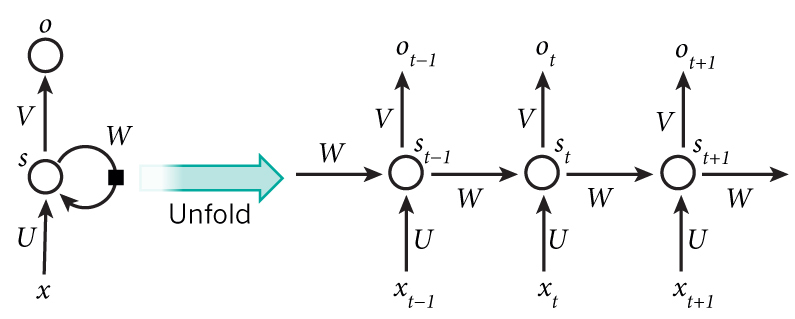
\includegraphics[scale = 0.5]{rnn-structure.jpg}
    \caption{RRN and the unfolding in time of the computation involved in its forward computation. Nguồn: Nature}
    \label{fig:fig1}
\end{figure}

Mô hình miêu tả ở Hình \ref{fig:fig1}, cho phép triển khai nội dung của một RNN với cấu trúc chuỗi tuần tự. Ví dụ ta có một câu gồm 4 từ "MaSSP thật thú vị" thì RNN sẽ được triển khai gồm 4 tầng nơ-ron tương ứng với mỗi từ một tầng. Việc tính toán cụ thể bên trong được thực hiện như sau:
\begin{itemize}
    \item $x_t$ là đầu vào tại bước $t$. Nếu sử dụng one-hot encode thì $x_t$ là vector one-hot tương ứng với từ nằm trong từ điển.
    \item $s_t$ là trạng thái ẩn tại bước $t$. Nó chính là bộ nhớ của mạng, xuyến suốt, tuần tự liên kết với nhau. $s_t$ được tính toán dựa trên đầu vào tại bước đó và trạng thái ẩn của bước trước\\
    $s_t = f(U \cdot x_t + W \cdot s_{t-1})$\\
    Hàm $f$ thường là một hàm non-linear như hàm tanh, hay ReLU. Để thực hiện được phép toán cho phần tử ẩn đầu tiên $s_0$ ta thường thêm vào phần tử $s_{-1}$, và khởi tạo cho nó giá trị bằng 0.
    \item $o_t$ là đầu ra tại bước $t$. Kết quả $o_t$ thường là vector xác suất các từ trong danh sách từ vựng của mình\\
    $o_t = softmax(V \cdot s_t)$
    
\end{itemize}

\section{Ứng dụng của RNN}
\subsection{Mô hình hóa ngôn ngữ và sinh văn bản}

Mô hình ngôn ngữ cho phép ta dự đoán được xác suất của một từ xuất hiện sau một chuỗi các từ ở phía trước nó. Điểm lý thú là từ đó chúng ta có thể xây dựng được một mô hình tự sinh từ cho phép máy tính có thể tạo ra các văn bản mới từ tập mẫu và xác suất đầu ra của mỗi từ. Do đó, tùy thuộc vào mô hình ngôn ngữ mà chúng ta có thể tạo ra nhiều văn bản khác nhau. \\
Trong mô hình ngôn ngữ, đầu vào thường là một chuỗi các từ và đầu ra là một chuỗi các từ dừ đoán được. Khi huấn luyện mạng, ta sẽ gán $o_t = x_{t+1}$ vì ta muốn đầu ra tại bước $t$ chính là từ tiếp theo của câu.

Một số nghiên cứu về mô hình hóa và sinh văn bản ứng dụng RNN:
\begin{itemize}
    \item Recurrent neural network based language model \cite{mikolov10}.
    \item Extensions of Recurrent neural network based language model \cite{mikolov11}.
    \item Generating Text with Recurrent Neural Networks \cite{sutskever11}.
\end{itemize}

\subsection{Machine Translation}
Machine Translation (Dịch máy) tương tự như mô hình hóa ngôn ngữ ở điểm đầu vào là chuỗi các từ trong ngôn ngữ nguồn cần dịch. Đầu ra sẽ là chuỗi các từ trong ngôn ngữ đích. Điểm khác nhau so với phương pháp ở trên là chúng ta chỉ xử lý sau khi đã xem xét toàn bộ chuỗi đầu vào. Vì từ dịch đầu tiên của câu cần phải có đầy đủ thông tin đầu vào cần dịch mới có thể suy luận, dịch chính xác được.
\begin{figure}[h]
    \centering
    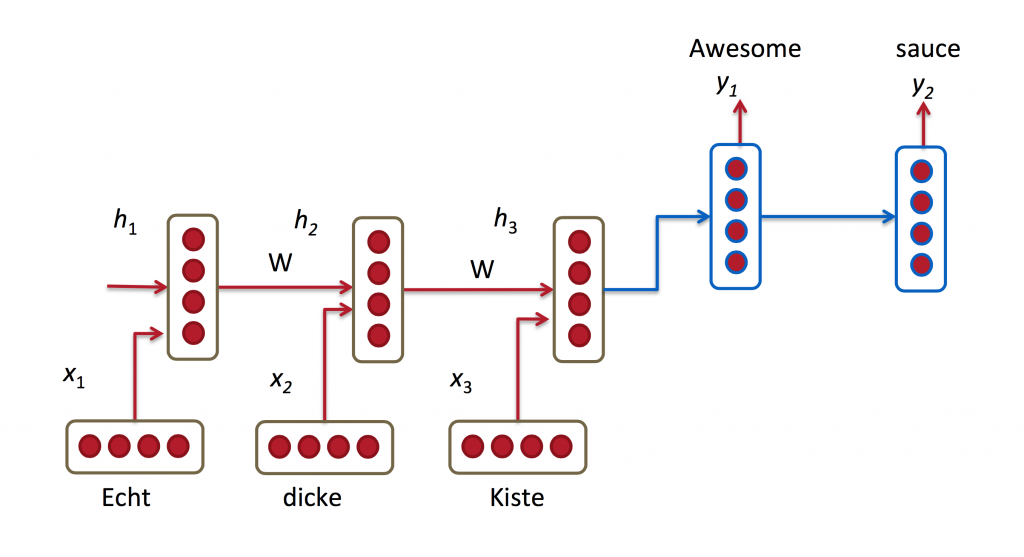
\includegraphics[scale = 0.5]{rnn-machine-translation.png}
    \caption{RNN for Machine Translation. Nguồn: CS224 Stanford}
    \label{fig:fig2}
\end{figure}
Một số nghiên cứu về machine translation ứng dụng RNN:
\begin{itemize}
    \item A Recursive Recurrent Neural Network for Statistical Machine Translation \cite{LiuYLZ14}.
    \item Sequence to Sequence Learning with Neural Networks \cite{SutskeverVL14}.
    \item Joint Language and Translation Modeling with Recurrent Neural Networks \cite{AuliGQZ13}.
\end{itemize}

\subsection{Huấn luyện RNN}
Huấn luyện mạng RNN cũng tương tự như các mạng neural truyền thống khác, tuy nhiên giải thuật lan truyền ngược (backpropagation) phải thay đổi một chút. Vì các tham số trong mạng RNN được sử dụng chung cho tất cả các bước trong mạng $(U, W, V)$ do đó đạo hàm tại mỗi đầu ra của các lớp trong RNN không chỉ phụ thuộc vào các tính toán tại bước đó, mà còn phụ thuộc vào các bước trước. Do đó để tính đạo hàm tại $t=3$ ta phải tính lan truyền ngược cả 2 bước phía trước rồi cộng tổng đạo hàm của chúng lại với nhau. Việc tính đạo hàm kiểu này được gọi là lan truyền ngược liên hồi (BPTT - Backpropagation Through Time).\\
Một lưu ý của việc huấn luyện RNN là khi các bước phụ thuộc càng xa thì càng dễ xuất hiện hiện tượng đạo hàm bị triệt tiêu (vanishing). LSTM đã được nghiên cứu để giải quyết vấn đề này của RNN truyền thống.

\printbibliography

\end{document}